\documentclass[journal,12pt,twocolumn]{IEEEtran}

\usepackage{setspace}
\usepackage{algpseudocode}
\usepackage{algorithm}
\usepackage{gensymb}
\singlespacing
\usepackage[cmex10]{amsmath}

\usepackage{amsthm}

\usepackage{mathrsfs}
\usepackage{txfonts}
\usepackage{stfloats}
\usepackage{bm}
\usepackage{cite}
\usepackage{cases}
\usepackage{subfig}
\usepackage{tikz}
\usepackage{longtable}
\usepackage{multirow}

\usepackage{enumitem}
\usepackage{mathtools}
\usepackage{steinmetz}
\usepackage{tikz}
\usepackage{circuitikz}
\usepackage{verbatim}
\usepackage{tfrupee}
\usepackage[breaklinks=true]{hyperref}
\usepackage{graphicx}
\usepackage{tkz-euclide}

\usetikzlibrary{calc,math}
\usepackage{listings}
    \usepackage{color}                                            %%
    \usepackage{array}                                            %%
    \usepackage{longtable}                                        %%
    \usepackage{calc}                                             %%
    \usepackage{multirow}                                         %%
    \usepackage{hhline}                                           %%
    \usepackage{ifthen}                                           %%
    \usepackage{lscape}     
\usepackage{multicol}
\usepackage{chngcntr}

\DeclareMathOperator*{\Res}{Res}

\renewcommand\thesection{\arabic{section}}
\renewcommand\thesubsection{\thesection.\arabic{subsection}}
\renewcommand\thesubsubsection{\thesubsection.\arabic{subsubsection}}

\renewcommand\thesectiondis{\arabic{section}}
\renewcommand\thesubsectiondis{\thesectiondis.\arabic{subsection}}
\renewcommand\thesubsubsectiondis{\thesubsectiondis.\arabic{subsubsection}}


\hyphenation{op-tical net-works semi-conduc-tor}
\def\inputGnumericTable{}                                 %%

\lstset{
%language=C,
frame=single, 
breaklines=true,
columns=fullflexible
}
\begin{document}


\newtheorem{theorem}{Theorem}[section]
\newtheorem{problem}{Problem}
\newtheorem{proposition}{Proposition}[section]
\newtheorem{lemma}{Lemma}[section]
\newtheorem{corollary}[theorem]{Corollary}
\newtheorem{example}{Example}[section]
\newtheorem{definition}[problem]{Definition}

\newcommand{\BEQA}{\begin{eqnarray}}
\newcommand{\EEQA}{\end{eqnarray}}
\newcommand{\define}{\stackrel{\triangle}{=}}
\bibliographystyle{IEEEtran}
\raggedbottom
\setlength{\parindent}{0pt}
\providecommand{\mbf}{\mathbf}
\providecommand{\pr}[1]{\ensuremath{\Pr\left(#1\right)}}
\providecommand{\qfunc}[1]{\ensuremath{Q\left(#1\right)}}
\providecommand{\sbrak}[1]{\ensuremath{{}\left[#1\right]}}
\providecommand{\lsbrak}[1]{\ensuremath{{}\left[#1\right.}}
\providecommand{\rsbrak}[1]{\ensuremath{{}\left.#1\right]}}
\providecommand{\brak}[1]{\ensuremath{\left(#1\right)}}
\providecommand{\lbrak}[1]{\ensuremath{\left(#1\right.}}
\providecommand{\rbrak}[1]{\ensuremath{\left.#1\right)}}
\providecommand{\cbrak}[1]{\ensuremath{\left\{#1\right\}}}
\providecommand{\lcbrak}[1]{\ensuremath{\left\{#1\right.}}
\providecommand{\rcbrak}[1]{\ensuremath{\left.#1\right\}}}
\theoremstyle{remark}
\newtheorem{rem}{Remark}
\newcommand{\sgn}{\mathop{\mathrm{sgn}}}
% \providecommand{\abs}[1]{\left\vert#1\right\vert}
% \providecommand{\res}[1]{\Res\displaylimits_{#1}} 
% \providecommand{\norm}[1]{\left\lVert#1\right\rVert}
% %\providecommand{\norm}[1]{\lVert#1\rVert}
% \providecommand{\mtx}[1]{\mathbf{#1}}
% \providecommand{\mean}[1]{E\left[ #1 \right]}
\providecommand{\fourier}{\overset{\mathcal{F}}{ \rightleftharpoons}}
%\providecommand{\hilbert}{\overset{\mathcal{H}}{ \rightleftharpoons}}
\providecommand{\system}{\overset{\mathcal{H}}{ \longleftrightarrow}}
	%\newcommand{\solution}[2]{\textbf{Solution:}{#1}}
\newcommand{\solution}{\noindent \textbf{Solution: }}
\newcommand{\cosec}{\,\text{cosec}\,}
\providecommand{\dec}[2]{\ensuremath{\overset{#1}{\underset{#2}{\gtrless}}}}
\newcommand{\myvec}[1]{\ensuremath{\begin{pmatrix}#1\end{pmatrix}}}
\newcommand{\mydet}[1]{\ensuremath{\begin{vmatrix}#1\end{vmatrix}}}
\numberwithin{equation}{subsection}
\def\putbox#1#2#3{\makebox[0in][l]{\makebox[#1][l]{}\raisebox{\baselineskip}[0in][0in]{\raisebox{#2}[0in][0in]{#3}}}}
     \def\rightbox#1{\makebox[0in][r]{#1}}
     \def\centbox#1{\makebox[0in]{#1}}
     \def\topbox#1{\raisebox{-\baselineskip}[0in][0in]{#1}}
     \def\midbox#1{\raisebox{-0.5\baselineskip}[0in][0in]{#1}}
\vspace{3cm}
\title{Assignment 1}
\author{Ritwik Sahani - EE18BTECH11038}
\maketitle
% \newpage
\bigskip
Github repository
%
\begin{lstlisting}
https://github.com/ritvix23/C-DataStructures/tree/master/Assignment1
\end{lstlisting}
\setcounter{figure}{0}
\section{Problem}
There are n unsorted arrays: A1 , A2 , …, An . Assume that n is odd. Each of A1 , A2 , …, An
contains n distinct elements. There are no common elements between any two arrays. The
worst-case time complexity of computing the median of the medians of A1 , A2 , …, An is -

\begin{enumerate}
    \item $O(n)$
    \item $O(nlogn)$
    \item  $O(n^{2})$
    \item $\Omega(n^{2}log n)$
\end{enumerate}



\section{Solution}
\subsection{Vagueness in question}
The question does not specify any algorithm for which the worst case is to be analyzed. Therefore, let us take two different algorithms, first brute force approach and then a comparatively efficient approach, and analyze worst cases for each one of them.


\subsection{Brute Force Approach}

Brute force approach involves sorting the arrays. After sorting, the task of finding the median of medians becomes trivial.
The exact steps are - 
\begin{itemize}
    \item Sort each array - $O(nlogn)$ for each array, $O(n^{2}logn)$ on the whole.
    \item Find the median of each sorted array - the element at  index $(n-1)/2$ (0-indexed) - for this left multiply the matrix with the following $1 \times n$ matrix ( that has one at $(n+1)/2$ and all other entries are zero)  - 

    \begin{center}
        
        $
        \begin{bmatrix}
            0 & 0 & . & . & 1 & . & . & 0 & 0 
        \end{bmatrix}
        $
        
    \end{center}

    
    \item This gives another $1 \times n$ matrix that contains the medians of the individual rows. 
    \item Sort this new matrix - $O(nlogn)$.
    \item Find the median of this new matrix by right mutiplying the matrix with the following $n \times 1 $ matrix (that has one at $(n+1)/2$ and all other entries are zero) - 
    
    \begin{center}
        

        $
        \begin{bmatrix}
            0\\
            0\\
            .\\
            .\\
            1\\
            .\\
            .\\
            0\\
            0\\
        \end{bmatrix}
        $
      
    \end{center}

    \item The resulting $1\times1$ matrix has just one entry which is the median of medians - $O(1)$.
\end{itemize}
Let us now analyze the time complexity of this approach - 
\newline

    $T(n) = O(n^{2}logn + n + nlogn + 1)$ 
    $\implies O(n^{2}logn)$


\subsection{Efficient Approach}
It should be intuitively clear that we are doing a lot of redundant work in sorting the arrays, while all we need is the middle element after sorting. Let us now look at an efficient approach to find this middle element without the need to sort the entire array. For a while, let us assume we have a routine - $qselect(k, array)$, that returns $k^{th}$ element, after sorting, in $array$ in linear time ($O(n)$).
Now, consider the following algorithm - 
    \begin{itemize}
        \item Use this routine on each array to find $n/2$ index element - basically the median of each array - $O(n)$ for each array, $O(n^{2})$ on the whole.
        \item Store these n medians in a separate array - $O(n)$
        \item Use the routine again on this new array to get median -  $O(n)$.
    \end{itemize} 


Let us now analyze the time complexity for this algorithm - 
\newline

    $T(n)  = O(n^{2} + n + n + 1)$
    $\implies O(n^{2})$

\subsection{Uncovering $qselect(.. , ..)$}

Let us see what we already know about this routine - 
    \begin{itemize}
        \item Parameters - number $k$, array $arr$ (possibly unsorted)
        \item Returns - $k^{th}$ index element in $arr$ after sorting.
        \item Should do the required job in linear time.
    \end{itemize}
    
The starting point to design such an algorithm is the following idea  - 
\newline
\textbf{Find which part of the array the required element might lie in, then truncate and recurse.
}

The exact algorithm consists of following steps - 
\begin{itemize}
    \item Choose a pivot element from the array (choose uniformly at random). 
    \item Partition the array so that all the elements less than the pivot element would lie on the left of the pivot element and all the elements greater than the pivot would lie on its right side after the partitioning - this can be done in O(n) by comparing and swapping other elements with pivot element. 
    \item After the prev step, the pivot would be exactly at the same index as it would if the array was sorted - call this index $i_{P}$.
    \item Now if $i_{P} = k \implies$ the element we are looking for is the pivot element, we are done, otherwise if $i_{P} >  k \implies$ lies in the sub-array on  the left to the pivot, in any other case it lies in the right sub-array. 
    \item Recurse on the appropriate sub-array determined from the prev step.
\end{itemize}

Pseudo code for qselect is as follows - 
\begin{algorithm}
\caption{QSELECT(A[0 .. n-1], k)}
\begin{algorithmic}
\If{$n$ is 1} 
    \State return A[0]
    
\Else 
    \State choose a pivot element A[p]
    \State $i_{P} \gets PARTITION(A[0..n-1], p)$
    \If{$k < i_{P}$}  
        \State return qselect(A[0..$i_{p}$-1], k)
    \ElsIf{$k > r$ } 
         \State return qselect(A[$i_{P}$+1..n-1], k - $i_{p}$)
    \Else  
        \State return A[$i_{P}$]
    \EndIf
\EndIf

\end{algorithmic}
\end{algorithm}

\begin{algorithm}
\caption{PARTITION(A[0 .. n-1], k)}
\begin{algorithmic}
    \State swap $A[p] \longleftrightarrow A[n]$ 
    \State $l \gets 0 $
    \For{\State $i \gets $0 to n-2}
        \If{$A[i]< A[n]$} 
        \State $l \gets l+1$
        \State swap $A[l] \longleftrightarrow A[i] $
        \EndIf
    \EndFor
    \State swap $A[n] \longleftrightarrow A[l+1]$
    \State return $l+1$

\end{algorithmic}
\end{algorithm}

Theoretical time complexity can be calculated from the recursive relation - \\
$T(N)  = T(N/2) + O(N)$ \\
$\implies T(N) = O(N)$ \\
the next section  verifies the theoretical results. 
\section{Verification}
To verify the theoretical results, I measured the execution times of both the algorithms and plotted them with the theoretical bounds - 

\begin{figure}[!h]
    \centering
    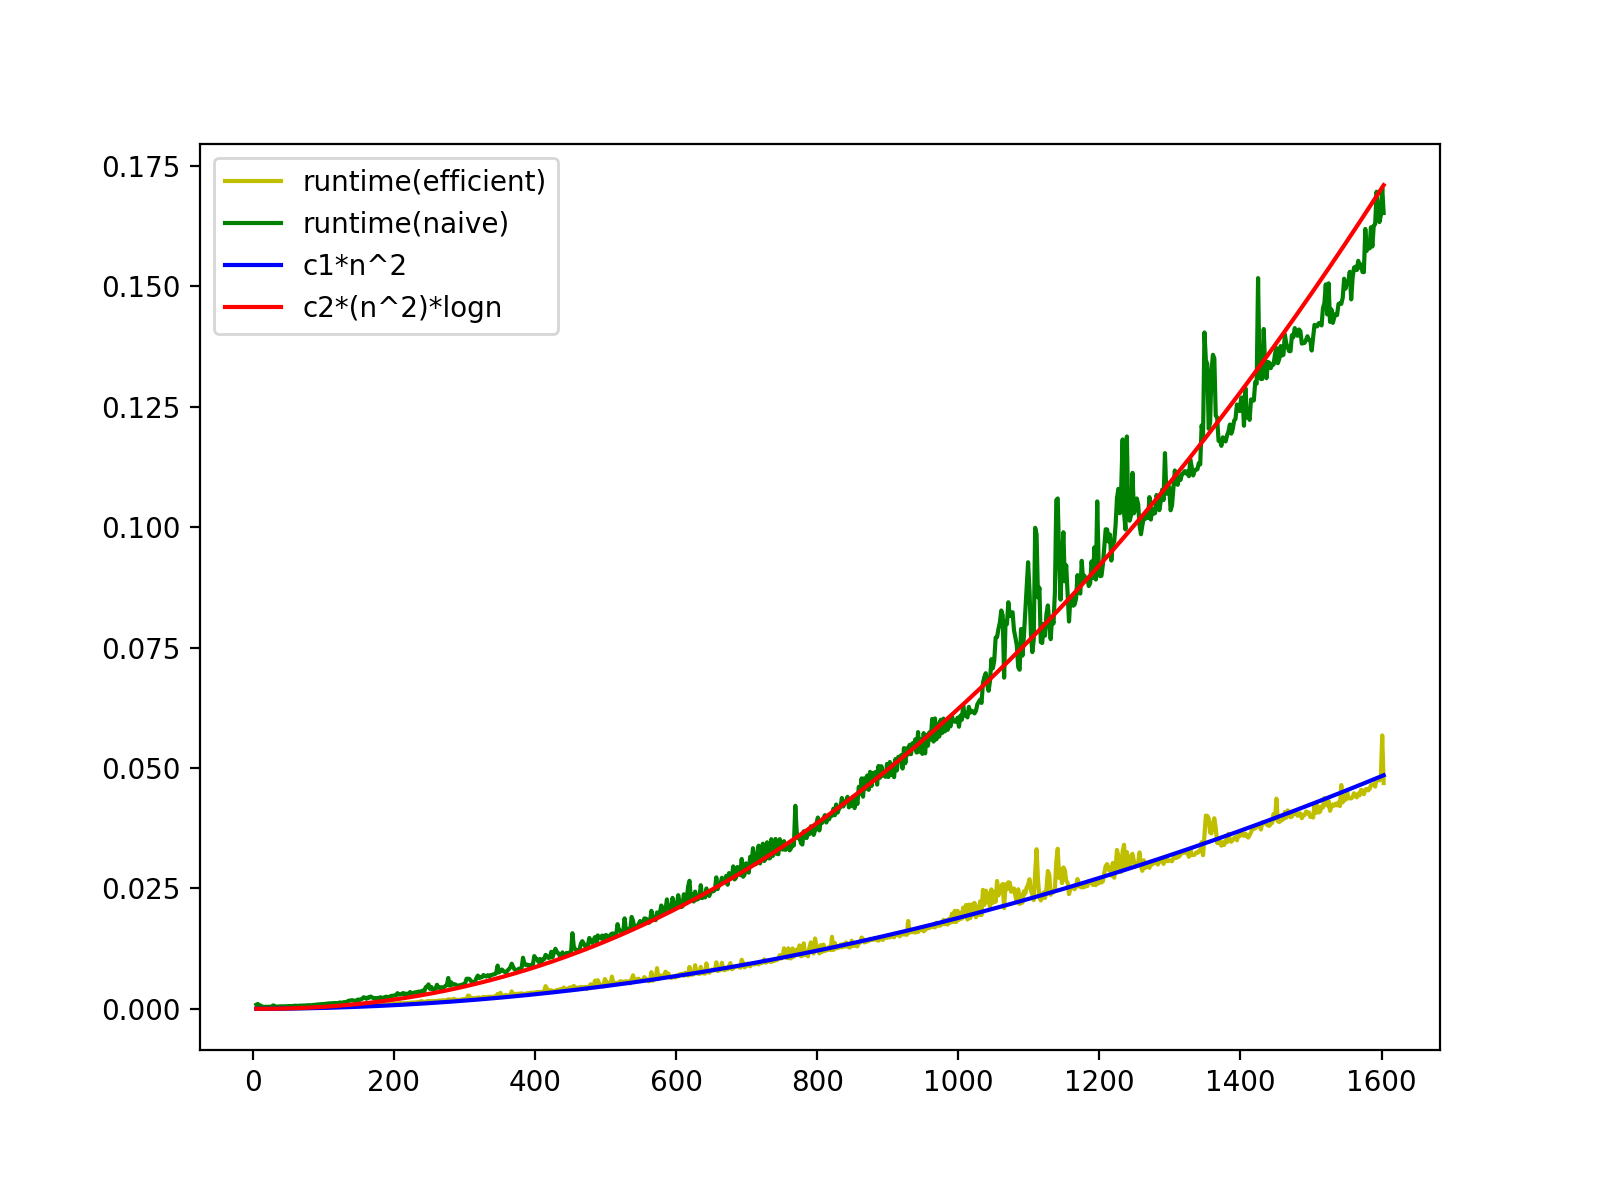
\includegraphics[scale=0.5]{plots/verification.png}
    \caption{Execution Times}
    \label{fig:verification}
\end{figure}

We can clearly observe that the execution times align with the theoretical findings.

This plot can be generated through the following python script
\begin{lstlisting}
https://github.com/ritvix23/C-DataStructures/blob/master/Assignment1/codes/timer.py
\end{lstlisting}
\end{document}